\documentclass{article}
\usepackage[utf8]{inputenc}
\usepackage[margin=1in]{geometry}
\usepackage{graphicx}
\usepackage{natbib}
\usepackage{enumitem}
\usepackage{array}
\usepackage{gensymb}
\usepackage{indentfirst}
\graphicspath{ {Images/} }
\usepackage{float}
\usepackage[table,xcdraw]{xcolor}
\usepackage{amsmath}

\title{Physics 111A Fall 2016- Lab 10\\Analog to Digital and Digital to Analog Conversion}
\author{Joshua Levy\\Lab Partner: Alex Chuang}
\date{November 13th, 2016}

\begin{document}

\maketitle

\section{Lab Write Up}
%1
\subsection{Aliasing and Sample Rate}
    See signature Page
    
%2
\subsection{Digital to Analog Conversion}
    \begin{figure}[H]
        \centering
        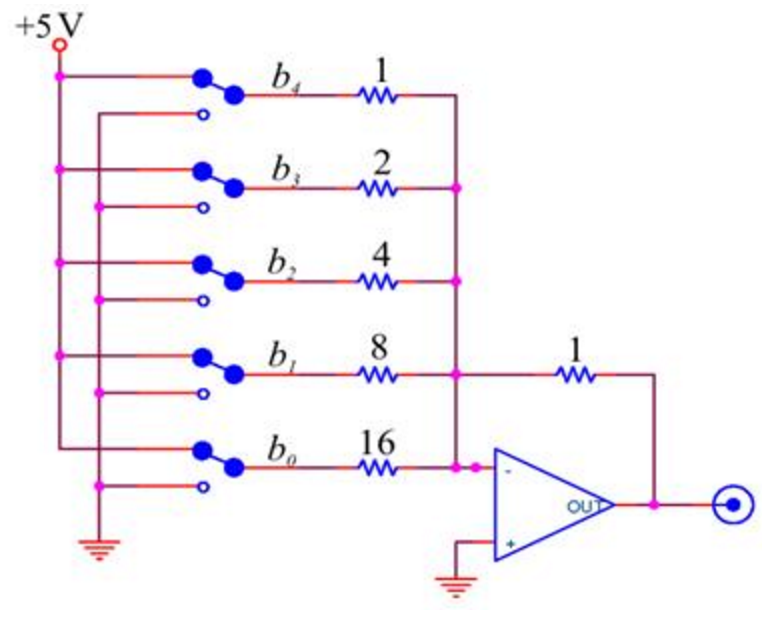
\includegraphics[scale = 0.5]{2a.png}
        \caption{DAC Converter \cite{lab10}}
        \label{fig:my_label}
    \end{figure}
    We constructed the above scaled resistor DAC. The values of resistors were produced such that the resistor titled "1", the lowest resistor, would have a max current of:
    \begin{equation}
        i_{max} = \frac{5V}{Z_{1}} = 2.5 mA
    \end{equation}
    Where $Z_1$ is the impedance of the lowest valued resistor in question. Through simple rearrangement, $Z_1 = 2k\Omega$. Thus, the 2 2k resistors were used in the circuit for the "1" resistors, a 4k resistor was used as the "2" resistor, an 8k resistor was used as the "4" resistor, and so on and so forth. These resistors were synthesized by using various combinations of 1$\%$ 1k and 10k resistors in series and parallel. \\\indent In the prelab, we found that our maximum output voltage should be 9.6875V. However, we built a LabVIEW driver for the DAQ as seen below:
    \begin{figure}[H]
        \centering
        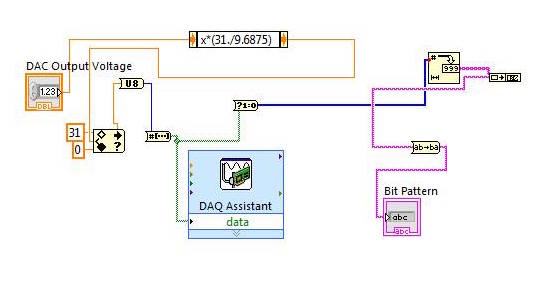
\includegraphics[scale = 0.5]{2b.jpeg}
        \caption{LabView Driver for DAC Code \cite{lab10}}
        \label{fig:my_label}
    \end{figure}
    and testing the DAC driver program by looking at outputs of the DAC from the oscilloscope. We saw that the oscilloscope put out voltages between 0 and roughly our max voltage, and our desired voltages roughly matched out measured voltages (save for the inversion gain factor of -1). The results are displayed in the following table: 
    \begin{table}[H]
        \centering
        \caption{Desired voltage plugging into LabView driving program vs. measured voltage in oscilloscope}
        \label{my-label}
        \begin{tabular}{ll}
        \textbf{$V_{desired}$ (V)} & \textbf{$V_{meas}$ (V)} \\ \hline
        1 & -1.1 \\
        2 & -2 \\
        3 & -3.15 \\
        4 & -4.1 \\
        9 & -8.91 \\
        -5 & -0.1 \\
        15 & -9.52
        \end{tabular}
        \end{table}
    Inputting values over our max DAC output were not allowed and resulted in only the maximum magnitude DAC output being displayed, and inputting desired values less than 0V resulted in an approximately 0V DAC output. And using our program from [1.3] (not shown), we plotted our desired DAC output voltage versus our actually found DAC output voltage:
    \begin{figure}[H]
        \centering
        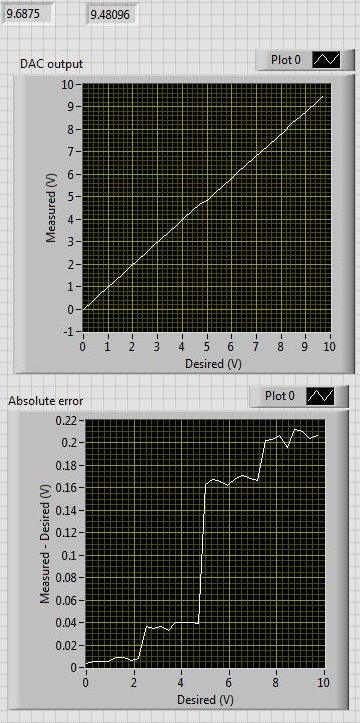
\includegraphics[scale = 0.5]{2c.jpeg}
        \caption{Desired voltage plugging into LabView driving program vs. measured voltage, and deviation graph through labview program developed in [1.3] \cite{lab10}}
        \label{fig:my_label}
    \end{figure}
    and we see that the maximum magnitude measured DAC output voltage is 9.481 V instead of 9.6875V. From the oscilloscope measured DAC output voltage data, we see that the maximum magnitude measured DAC output voltage is 9.52 V instead of 9.6875V.
    
    
%3
\subsection{}
    See signature page
    
%4
\subsection{Analog to Digital Conversion}
    \begin{figure}[H]
        \centering
        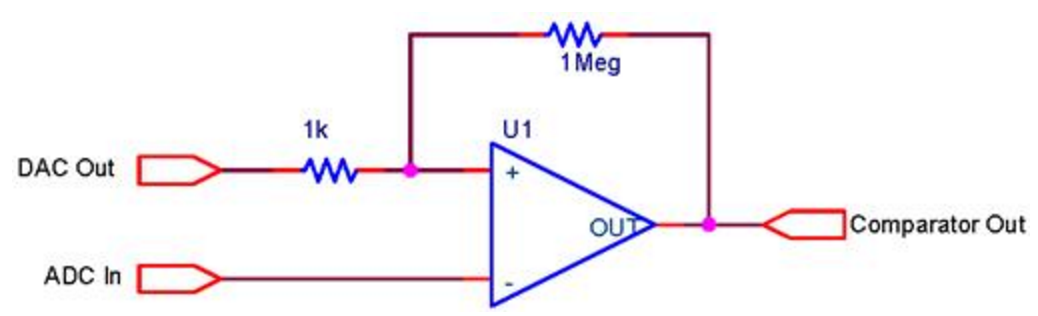
\includegraphics[scale = 0.5]{4a.png}
        \caption{Comparator to compare DAC output with ADC input \cite{lab10}}
        \label{fig:my_label}
    \end{figure}
    We built a successive approximation ADC by adding a comparator to the DAC output. The ADC made successive guesses to try to get close to the DAC output using some code that was developed below.\\\indent First, we constructed the program "Compare Trial.vi", which compared the DAC output to a fixed voltage using a comparator. If the comparator output was positive, our program would display a true reading, and if the comparator output was negative, a false reading would display. Pictured below is our code:
    \begin{figure}[H]
        \centering
        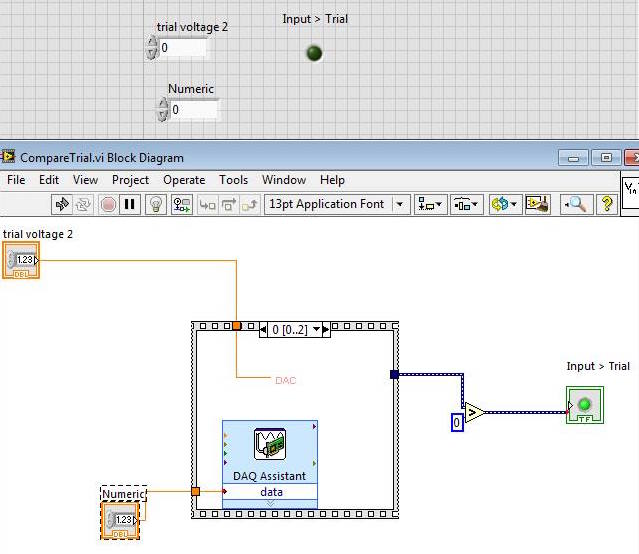
\includegraphics[scale = 0.5]{4b.jpeg}
        \caption{"Compare Trial.vi" code \cite{lab10}(citing the lab and another group in our class who we designed the program with; there were not enough seats in lab class that day and the GSIs gave us permission to collaborate on this program)}
        \label{fig:my_label}
    \end{figure}
    We added features of the above code to our program "ADC.vi", which compares the ADC output to the DAC output and makes new ADC guesses that are closer to the DAC output until the ADC voltage begins to converge on the DAC output. The code is pictured below:
    \begin{figure}[H]
        \centering
        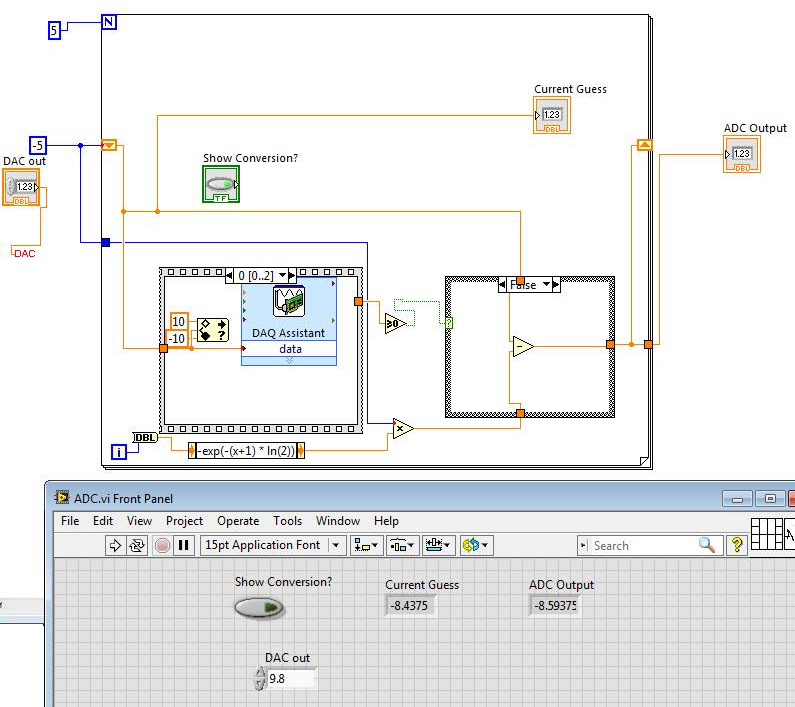
\includegraphics[scale = 0.5]{4c.png}
        \caption{"ADC.vi" code, 2 parts of stacked sequence structure not shown \cite{lab10}}
        \label{fig:my_label}
    \end{figure}
    After running a few trials, we see that (using the routine we designed in [1.5], which iterates the ADC successive approximation over 64 DAC outputs between 0V and 8.66V): 
    \begin{figure}[H]
        \centering
        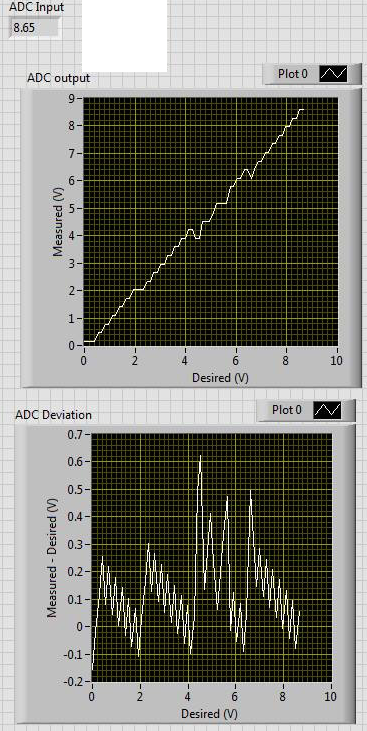
\includegraphics[scale = 0.5]{etc.png}
        \caption{ADC output, measured vs. desired, using program from [1.5] \cite{lab10}}
        \label{fig:my_label}
    \end{figure}
    And the ADC seems to converge quite well to the DAC output for its range of minimum to maximum possible DAC output voltages. In this section, we used a new DAQ card to conduct the study, and found that the voltages leaving the pins on the DAQ card digital output were different from the ones that yielded a 9.48V max DAC output. Thus, the new maximum DAC output was 8.66V, reflected in the figure below, using the [1.3] routine to find the total range of DAC outputs. We incorporated this new maximum output in our "ADC.vi" to display input and output values between 0V, and the new maximum DAC output of 8.66V:
    \begin{figure}[H]
        \centering
        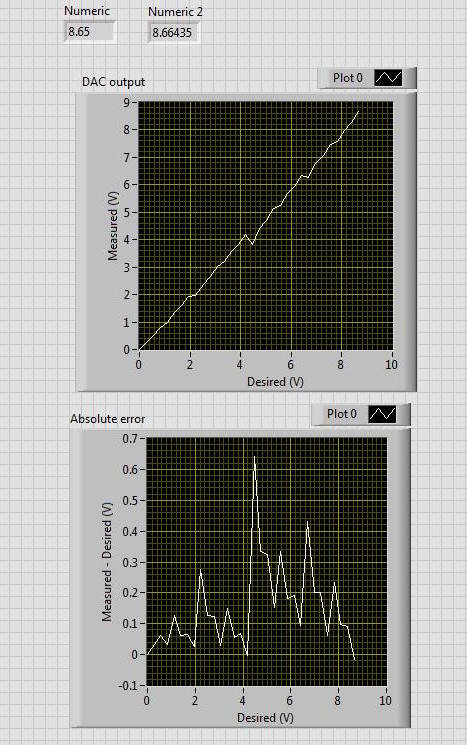
\includegraphics[scale = 0.5]{4d.jpeg}
        \caption{New DAC measured vs. desired data; new max DAC output \cite{lab10}}
        \label{fig:my_label}
    \end{figure}
    
%5
\subsection{}
    See signature page
    
%6
\subsection{}
    We ran the routine "Test DAQ ADC and DAC.vi" to test the accuracy of the DAQ converter. We see that the value of one bit is (given that the voltage ranged between -10V and 10V and there were $2^{12}$ possible discrete voltage values that could be taken on for a 12-bit converter):
    \begin{equation}
        1 bit = \frac{20V}{2^{12}} \approx 0.004883 V
    \end{equation}
    We ran the routine, and produced the graphs below:
    \begin{figure}[H]
        \centering
        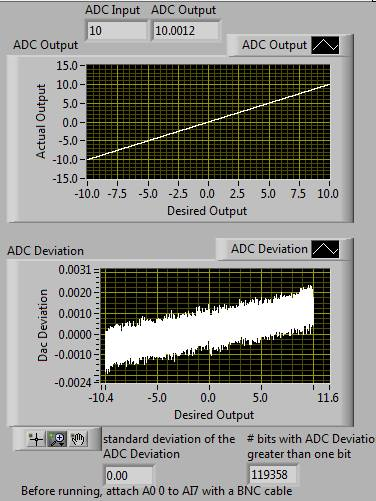
\includegraphics[scale = 0.5]{6a.png}
        \caption{DAQ Converter Accuracy Test, ADC actual output vs desired output and ADC/DAC deviation graph \cite{lab10}}
        \label{fig:my_label}
    \end{figure}
    We looked to see where the DAC deviation was greater than 1 bit (=0.0049V), and we saw that most deviations were under 0.002V magnitude. Thus, there were no DAC errors larger than 1 bit.
    
    
    
%7
\subsection{}
    We used the program "Sine$\_$DAQ$\_$Drive.vi" to output a 5V sine wave on the analog output. We adjusted the drive frequency, and found that the signal is acceptable when the frequency is at or below 100$\Omega$, or else the signal begins to resemble a step function and begins to look less like a sine wave (more like squarish stepwise output, figure 10e).\\\indent Now we used 3.3k resistors to "construct simple low pass filters with cut off frequencies near 10kHz and 1kHz" \cite{lab10} (we used a 4.8 nF capacitor for the 10kHz low pass filter and a 48.23 nF capacitor for the 1kHz low pass filter, utilizing the relationship $C=\frac{1}{2\pi f_{3dB}*R}$, where R is the 3.3k resistor and f is the cutoff frequency), and we display the output waveforms of the DAQ at various frequencies for the two filters and without a filter:
    \begin{figure}[H]
        \centering
        a)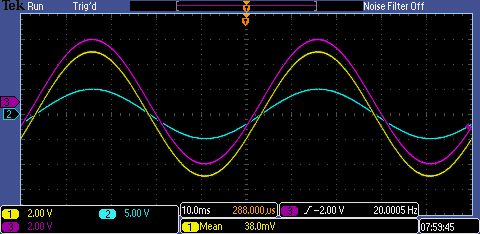
\includegraphics[scale = 0.4]{7a.PNG}
        b)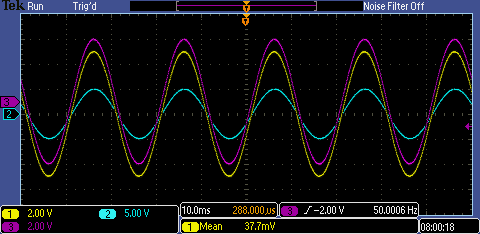
\includegraphics[scale = 0.4]{7b.PNG}
        c)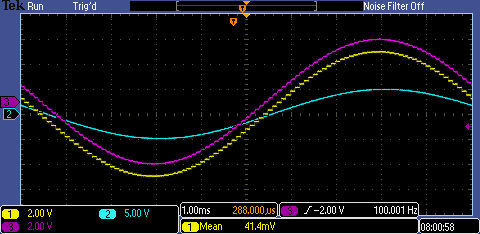
\includegraphics[scale = 0.4]{7c.PNG}
        d)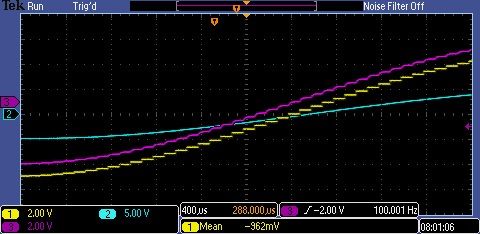
\includegraphics[scale = 0.4]{7d.PNG}
        e)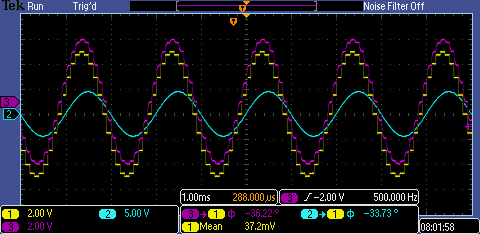
\includegraphics[scale = 0.4]{7e.PNG}
        f)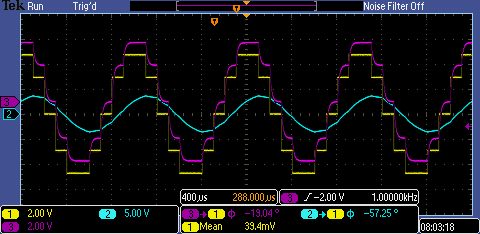
\includegraphics[scale = 0.4]{7f.PNG}
        g)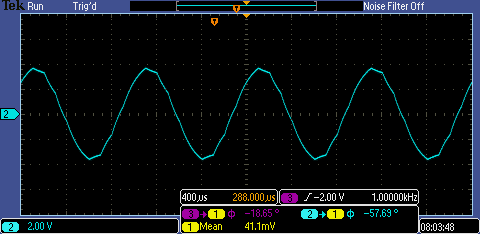
\includegraphics[scale = 0.4]{7g.PNG}
        h)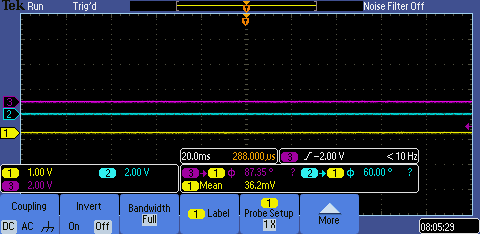
\includegraphics[scale = 0.4]{7h.PNG}
        \caption{Output of DAQ 5V sine wave using: no filter (yellow), 1kHz low pass filter (purple), and 10kHz filter (blue) for sine wave frequencies of: a)20 Hz, b)50Hz, c)100Hz, d)100Hz, e)500Hz, f) 1kHz, g) 5000kHz \cite{lab10}}
        \label{fig:my_label}
    \end{figure}
    Driving the filters/ no filter with a DAQ output, and the nyquist frequency is reached when f = 5kHz (figure 10h), killing the signals. \\\indent 
    We see that the 1kHz filter outperforms the 10kHz and no filter by significantly smoothing out the digital output signals. The 1kHz high pass filter produces an acceptable signal from very low driving frequencies (close to 0V) to at least 1kHz (figure 10g, where the output begins to look more piecewise). The 10kHz filter produces an acceptable signal from very low frequencies to somewhere between 100 and 500Hz. Because the low pass cutoff is so high for this filter, it does not experience the same smoothing effects that the 1kHz filter experiences. It resembles an output that almost looks like tiny charging and discharging capacitor outputs on a squarish wave (the purple output looks like capacitor charge/discharges for the yellow output). We see that as the frequency begins to increase, the 1kHz filter output (blue) begins to attenuate and experiences phase shifts more rapidly than the 10kHz filter, which remains more or less roughly in phase with the yellow DAQ-driven sine wave.




\section{Signature Page}
\begin{figure}[H]
    \centering
    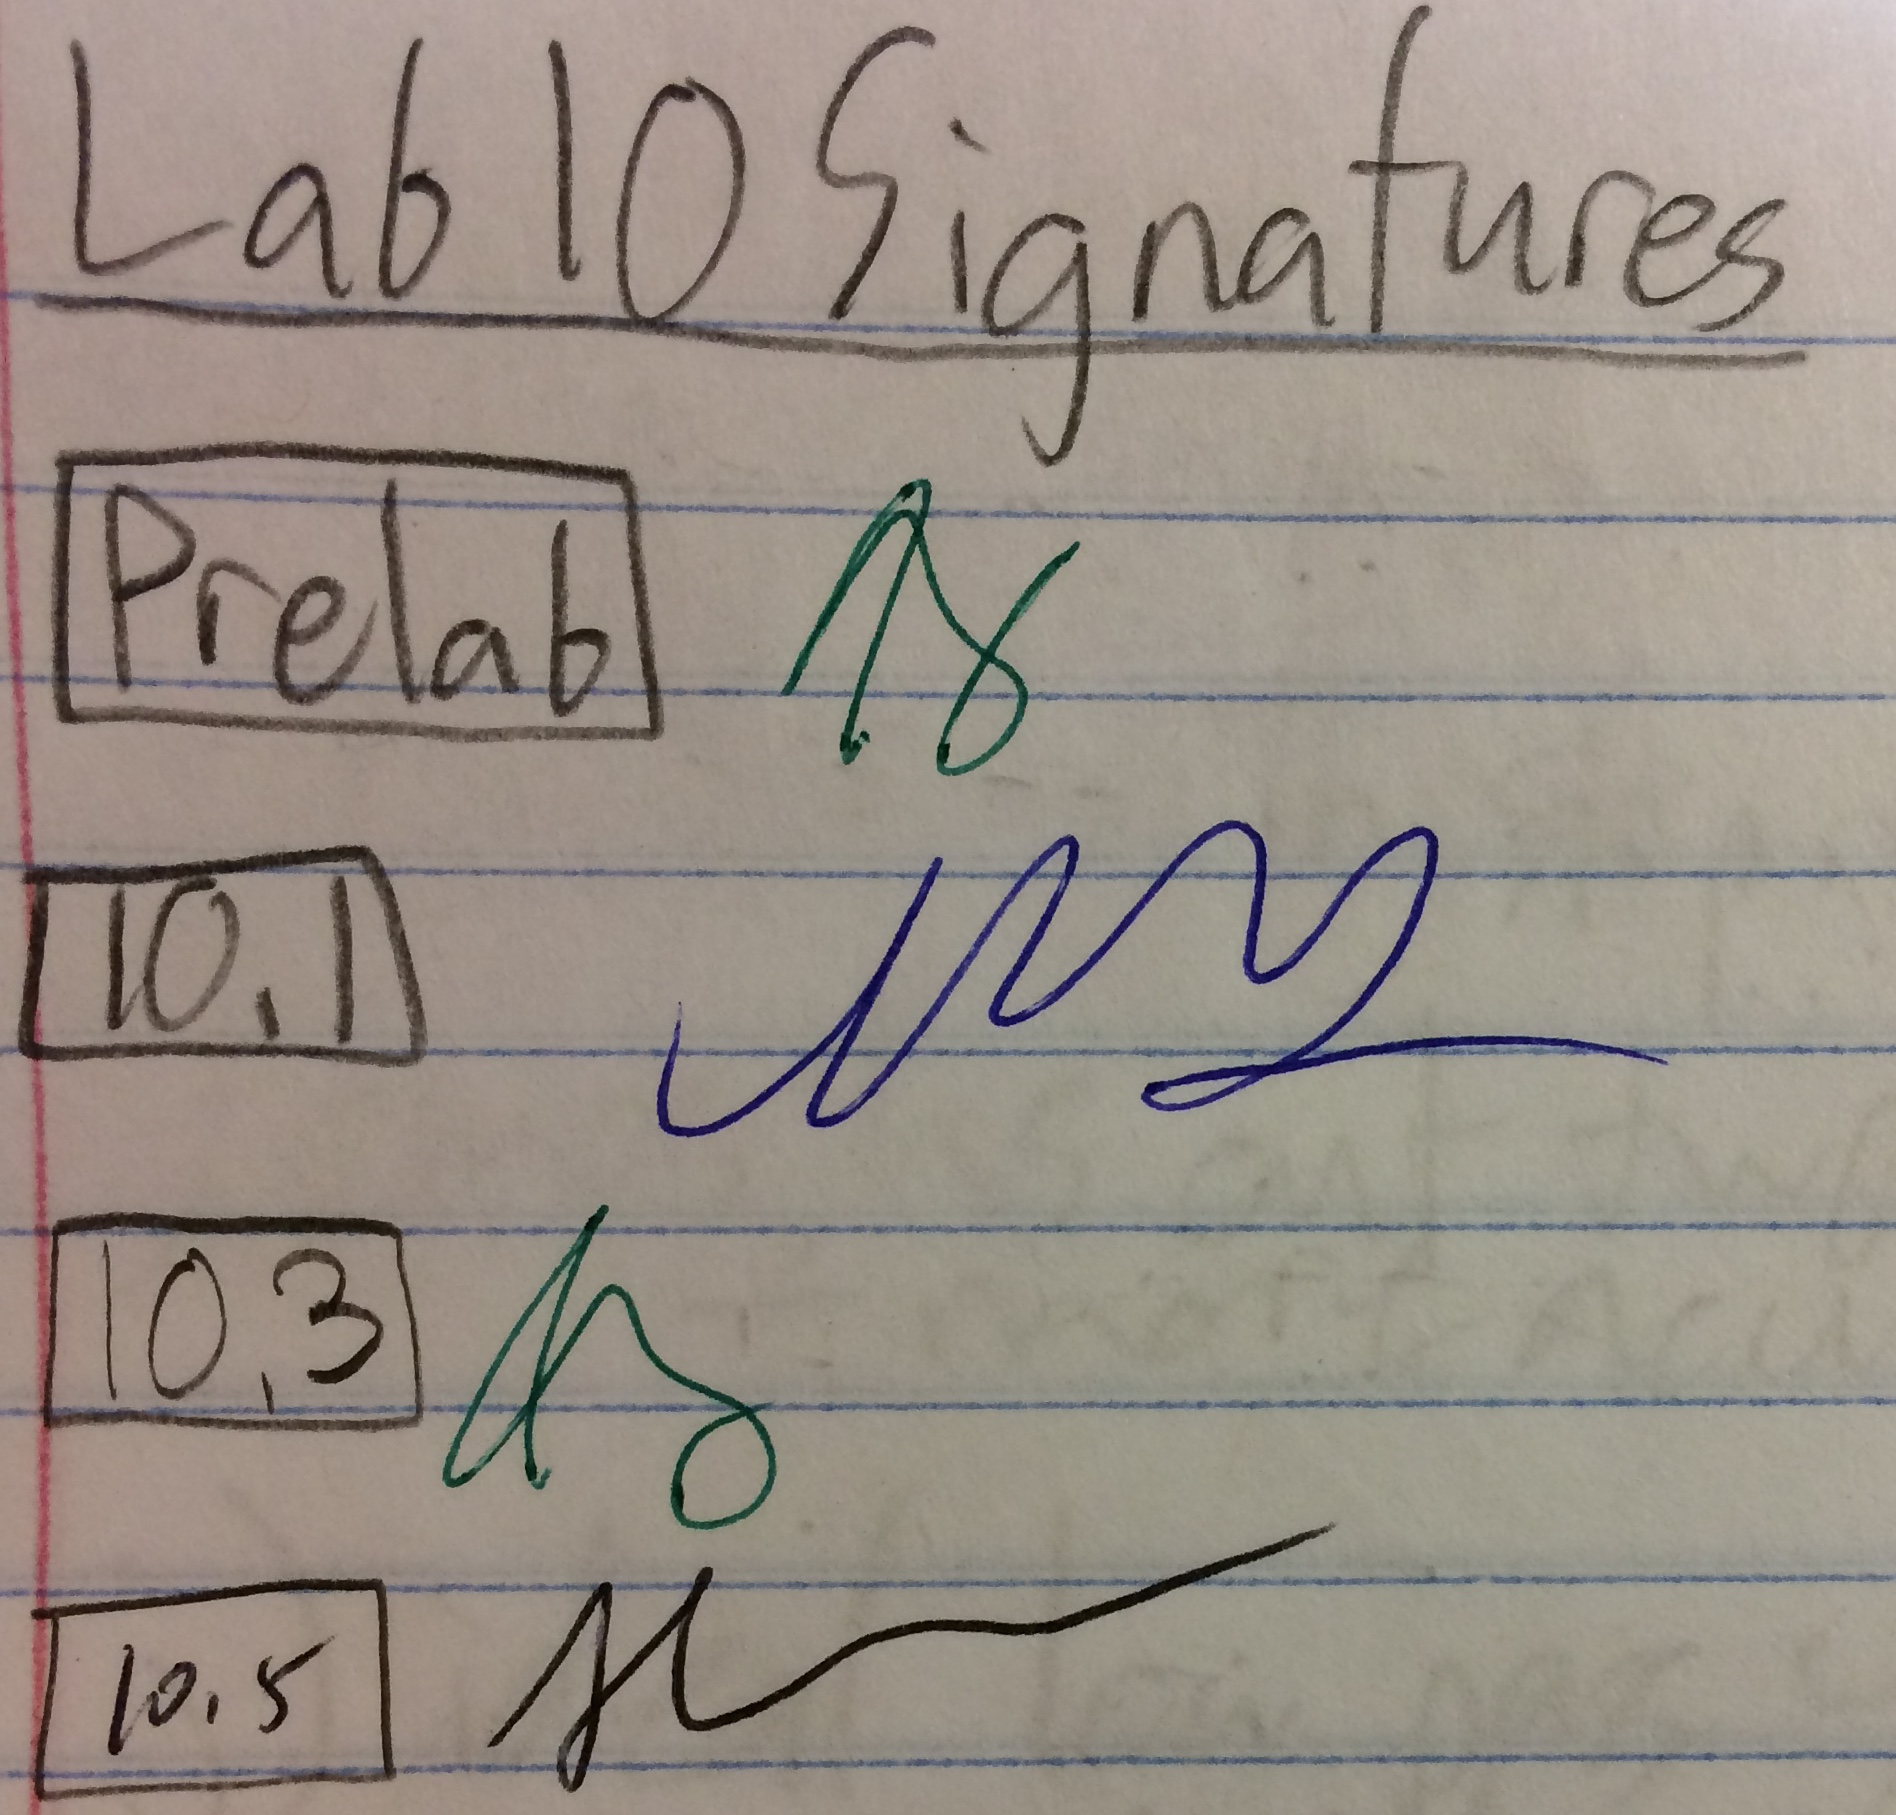
\includegraphics[scale = 0.15]{sig.JPG}
    \caption{Signatures}
    \label{fig:my_label}
\end{figure}



\bibliography{joshbib}{}
\bibliographystyle{plain}


\end{document}

\begin{figure}[H]
    \centering
    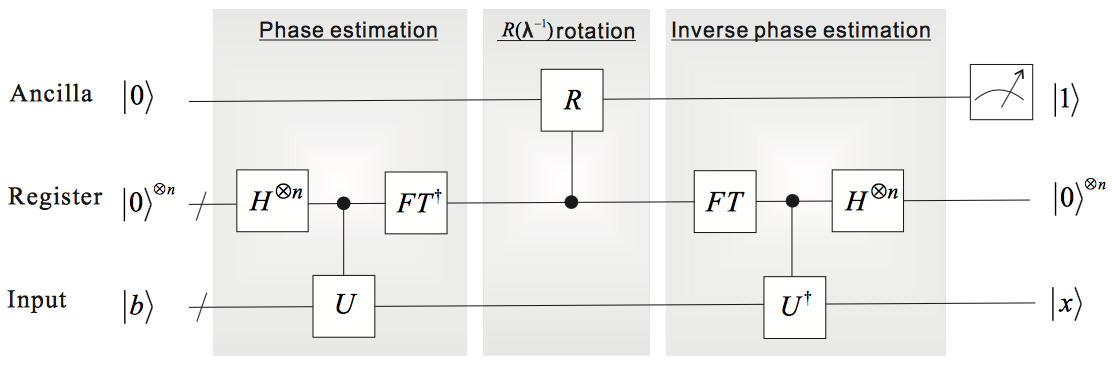
\includegraphics[scale = 0.5]{1.png}
    \caption{Caption \cite{lab10}}
    \label{fig:my_label}
\end{figure}

Todo:  images of working program 1.2, some of our test results 1.4, pictures of all three programs and their code, 1.6 qs, figures, equations, labels